\mode<article>{\usepackage{fullpage}}
\mode<presentation>{\usetheme{shurain}}


\usepackage{kotex}
\usepackage{multirow}
\usepackage{tikz}
\usepackage{graphicx}
\usepackage[normal, tight, center]{subfigure}
\usepackage{amssymb}
\usepackage{pgf}
\usepackage{url}
\usepackage{mathrsfs}
\usepackage{mathtools}
\usepackage{algorithm2e}
\usepackage{setspace}
\usepackage{fancyvrb}


\DeclareMathOperator*{\argmin}{\arg\!\min}
\DeclareMathOperator*{\argmax}{\arg\!\max}

\usepackage{fancyvrb}
\usepackage{color}

\makeatletter
\def\PY@reset{\let\PY@it=\relax \let\PY@bf=\relax%
    \let\PY@ul=\relax \let\PY@tc=\relax%
    \let\PY@bc=\relax \let\PY@ff=\relax}
\def\PY@tok#1{\csname PY@tok@#1\endcsname}
\def\PY@toks#1+{\ifx\relax#1\empty\else%
    \PY@tok{#1}\expandafter\PY@toks\fi}
\def\PY@do#1{\PY@bc{\PY@tc{\PY@ul{%
    \PY@it{\PY@bf{\PY@ff{#1}}}}}}}
\def\PY#1#2{\PY@reset\PY@toks#1+\relax+\PY@do{#2}}

\expandafter\def\csname PY@tok@gd\endcsname{\def\PY@tc##1{\textcolor[rgb]{0.63,0.00,0.00}{##1}}}
\expandafter\def\csname PY@tok@gu\endcsname{\let\PY@bf=\textbf\def\PY@tc##1{\textcolor[rgb]{0.50,0.00,0.50}{##1}}}
\expandafter\def\csname PY@tok@gt\endcsname{\def\PY@tc##1{\textcolor[rgb]{0.00,0.25,0.82}{##1}}}
\expandafter\def\csname PY@tok@gs\endcsname{\let\PY@bf=\textbf}
\expandafter\def\csname PY@tok@gr\endcsname{\def\PY@tc##1{\textcolor[rgb]{1.00,0.00,0.00}{##1}}}
\expandafter\def\csname PY@tok@cm\endcsname{\let\PY@it=\textit\def\PY@tc##1{\textcolor[rgb]{0.25,0.50,0.50}{##1}}}
\expandafter\def\csname PY@tok@vg\endcsname{\def\PY@tc##1{\textcolor[rgb]{0.10,0.09,0.49}{##1}}}
\expandafter\def\csname PY@tok@m\endcsname{\def\PY@tc##1{\textcolor[rgb]{0.40,0.40,0.40}{##1}}}
\expandafter\def\csname PY@tok@mh\endcsname{\def\PY@tc##1{\textcolor[rgb]{0.40,0.40,0.40}{##1}}}
\expandafter\def\csname PY@tok@go\endcsname{\def\PY@tc##1{\textcolor[rgb]{0.50,0.50,0.50}{##1}}}
\expandafter\def\csname PY@tok@ge\endcsname{\let\PY@it=\textit}
\expandafter\def\csname PY@tok@vc\endcsname{\def\PY@tc##1{\textcolor[rgb]{0.10,0.09,0.49}{##1}}}
\expandafter\def\csname PY@tok@il\endcsname{\def\PY@tc##1{\textcolor[rgb]{0.40,0.40,0.40}{##1}}}
\expandafter\def\csname PY@tok@cs\endcsname{\let\PY@it=\textit\def\PY@tc##1{\textcolor[rgb]{0.25,0.50,0.50}{##1}}}
\expandafter\def\csname PY@tok@cp\endcsname{\def\PY@tc##1{\textcolor[rgb]{0.74,0.48,0.00}{##1}}}
\expandafter\def\csname PY@tok@gi\endcsname{\def\PY@tc##1{\textcolor[rgb]{0.00,0.63,0.00}{##1}}}
\expandafter\def\csname PY@tok@gh\endcsname{\let\PY@bf=\textbf\def\PY@tc##1{\textcolor[rgb]{0.00,0.00,0.50}{##1}}}
\expandafter\def\csname PY@tok@ni\endcsname{\let\PY@bf=\textbf\def\PY@tc##1{\textcolor[rgb]{0.60,0.60,0.60}{##1}}}
\expandafter\def\csname PY@tok@nl\endcsname{\def\PY@tc##1{\textcolor[rgb]{0.63,0.63,0.00}{##1}}}
\expandafter\def\csname PY@tok@nn\endcsname{\let\PY@bf=\textbf\def\PY@tc##1{\textcolor[rgb]{0.00,0.00,1.00}{##1}}}
\expandafter\def\csname PY@tok@no\endcsname{\def\PY@tc##1{\textcolor[rgb]{0.53,0.00,0.00}{##1}}}
\expandafter\def\csname PY@tok@na\endcsname{\def\PY@tc##1{\textcolor[rgb]{0.49,0.56,0.16}{##1}}}
\expandafter\def\csname PY@tok@nb\endcsname{\def\PY@tc##1{\textcolor[rgb]{0.00,0.50,0.00}{##1}}}
\expandafter\def\csname PY@tok@nc\endcsname{\let\PY@bf=\textbf\def\PY@tc##1{\textcolor[rgb]{0.00,0.00,1.00}{##1}}}
\expandafter\def\csname PY@tok@nd\endcsname{\def\PY@tc##1{\textcolor[rgb]{0.67,0.13,1.00}{##1}}}
\expandafter\def\csname PY@tok@ne\endcsname{\let\PY@bf=\textbf\def\PY@tc##1{\textcolor[rgb]{0.82,0.25,0.23}{##1}}}
\expandafter\def\csname PY@tok@nf\endcsname{\def\PY@tc##1{\textcolor[rgb]{0.00,0.00,1.00}{##1}}}
\expandafter\def\csname PY@tok@si\endcsname{\let\PY@bf=\textbf\def\PY@tc##1{\textcolor[rgb]{0.73,0.40,0.53}{##1}}}
\expandafter\def\csname PY@tok@s2\endcsname{\def\PY@tc##1{\textcolor[rgb]{0.73,0.13,0.13}{##1}}}
\expandafter\def\csname PY@tok@vi\endcsname{\def\PY@tc##1{\textcolor[rgb]{0.10,0.09,0.49}{##1}}}
\expandafter\def\csname PY@tok@nt\endcsname{\let\PY@bf=\textbf\def\PY@tc##1{\textcolor[rgb]{0.00,0.50,0.00}{##1}}}
\expandafter\def\csname PY@tok@nv\endcsname{\def\PY@tc##1{\textcolor[rgb]{0.10,0.09,0.49}{##1}}}
\expandafter\def\csname PY@tok@s1\endcsname{\def\PY@tc##1{\textcolor[rgb]{0.73,0.13,0.13}{##1}}}
\expandafter\def\csname PY@tok@sh\endcsname{\def\PY@tc##1{\textcolor[rgb]{0.73,0.13,0.13}{##1}}}
\expandafter\def\csname PY@tok@sc\endcsname{\def\PY@tc##1{\textcolor[rgb]{0.73,0.13,0.13}{##1}}}
\expandafter\def\csname PY@tok@sx\endcsname{\def\PY@tc##1{\textcolor[rgb]{0.00,0.50,0.00}{##1}}}
\expandafter\def\csname PY@tok@bp\endcsname{\def\PY@tc##1{\textcolor[rgb]{0.00,0.50,0.00}{##1}}}
\expandafter\def\csname PY@tok@c1\endcsname{\let\PY@it=\textit\def\PY@tc##1{\textcolor[rgb]{0.25,0.50,0.50}{##1}}}
\expandafter\def\csname PY@tok@kc\endcsname{\let\PY@bf=\textbf\def\PY@tc##1{\textcolor[rgb]{0.00,0.50,0.00}{##1}}}
\expandafter\def\csname PY@tok@c\endcsname{\let\PY@it=\textit\def\PY@tc##1{\textcolor[rgb]{0.25,0.50,0.50}{##1}}}
\expandafter\def\csname PY@tok@mf\endcsname{\def\PY@tc##1{\textcolor[rgb]{0.40,0.40,0.40}{##1}}}
\expandafter\def\csname PY@tok@err\endcsname{\def\PY@bc##1{\setlength{\fboxsep}{0pt}\fcolorbox[rgb]{1.00,0.00,0.00}{1,1,1}{\strut ##1}}}
\expandafter\def\csname PY@tok@kd\endcsname{\let\PY@bf=\textbf\def\PY@tc##1{\textcolor[rgb]{0.00,0.50,0.00}{##1}}}
\expandafter\def\csname PY@tok@ss\endcsname{\def\PY@tc##1{\textcolor[rgb]{0.10,0.09,0.49}{##1}}}
\expandafter\def\csname PY@tok@sr\endcsname{\def\PY@tc##1{\textcolor[rgb]{0.73,0.40,0.53}{##1}}}
\expandafter\def\csname PY@tok@mo\endcsname{\def\PY@tc##1{\textcolor[rgb]{0.40,0.40,0.40}{##1}}}
\expandafter\def\csname PY@tok@kn\endcsname{\let\PY@bf=\textbf\def\PY@tc##1{\textcolor[rgb]{0.00,0.50,0.00}{##1}}}
\expandafter\def\csname PY@tok@mi\endcsname{\def\PY@tc##1{\textcolor[rgb]{0.40,0.40,0.40}{##1}}}
\expandafter\def\csname PY@tok@gp\endcsname{\let\PY@bf=\textbf\def\PY@tc##1{\textcolor[rgb]{0.00,0.00,0.50}{##1}}}
\expandafter\def\csname PY@tok@o\endcsname{\def\PY@tc##1{\textcolor[rgb]{0.40,0.40,0.40}{##1}}}
\expandafter\def\csname PY@tok@kr\endcsname{\let\PY@bf=\textbf\def\PY@tc##1{\textcolor[rgb]{0.00,0.50,0.00}{##1}}}
\expandafter\def\csname PY@tok@s\endcsname{\def\PY@tc##1{\textcolor[rgb]{0.73,0.13,0.13}{##1}}}
\expandafter\def\csname PY@tok@kp\endcsname{\def\PY@tc##1{\textcolor[rgb]{0.00,0.50,0.00}{##1}}}
\expandafter\def\csname PY@tok@w\endcsname{\def\PY@tc##1{\textcolor[rgb]{0.73,0.73,0.73}{##1}}}
\expandafter\def\csname PY@tok@kt\endcsname{\def\PY@tc##1{\textcolor[rgb]{0.69,0.00,0.25}{##1}}}
\expandafter\def\csname PY@tok@ow\endcsname{\let\PY@bf=\textbf\def\PY@tc##1{\textcolor[rgb]{0.67,0.13,1.00}{##1}}}
\expandafter\def\csname PY@tok@sb\endcsname{\def\PY@tc##1{\textcolor[rgb]{0.73,0.13,0.13}{##1}}}
\expandafter\def\csname PY@tok@k\endcsname{\let\PY@bf=\textbf\def\PY@tc##1{\textcolor[rgb]{0.00,0.50,0.00}{##1}}}
\expandafter\def\csname PY@tok@se\endcsname{\let\PY@bf=\textbf\def\PY@tc##1{\textcolor[rgb]{0.73,0.40,0.13}{##1}}}
\expandafter\def\csname PY@tok@sd\endcsname{\let\PY@it=\textit\def\PY@tc##1{\textcolor[rgb]{0.73,0.13,0.13}{##1}}}

\def\PYZbs{\char`\\}
\def\PYZus{\char`\_}
\def\PYZob{\char`\{}
\def\PYZcb{\char`\}}
\def\PYZca{\char`\^}
\def\PYZam{\char`\&}
\def\PYZlt{\char`\<}
\def\PYZgt{\char`\>}
\def\PYZsh{\char`\#}
\def\PYZpc{\char`\%}
\def\PYZdl{\char`\$}
\def\PYZti{\char`\~}
% for compatibility with earlier versions
\def\PYZat{@}
\def\PYZlb{[}
\def\PYZrb{]}
\makeatother


\setbeamercovered{transparent}

\def\supertiny{ \font\supertinyfont = cmr10 at 7pt \relax \supertinyfont}


\title[\hspace{2em}\insertframenumber/\inserttotalframenumber]{SK Planet Code Sprint 2013 Round 2}
\author[Sungjoo Ha]{Sungjoo Ha \\ @shurain{\Huge \_}}
\date{September 27th, 2013}

\institute{
    SNU Optimization and Financial Engineering Lab
}

\begin{document}

\frame {
\maketitle
}


\section{About Me}

\frame {
    \frametitle{하성주 (shurain)}
    \begin{columns}[t]
        \begin{column}[T]{5cm}
            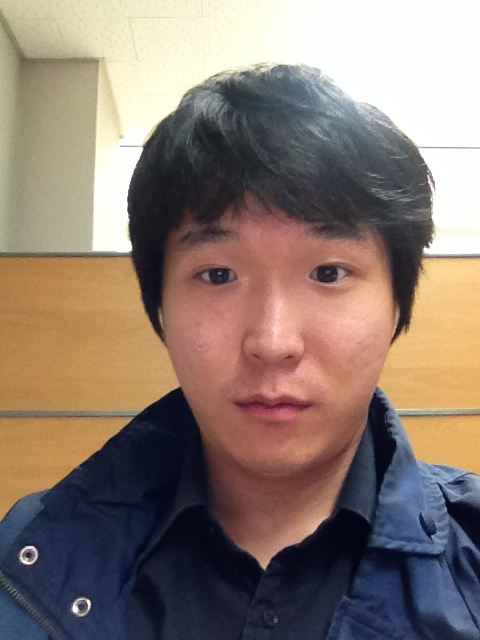
\includegraphics[height=0.8\paperheight]{shurain}
        \end{column}
        \begin{column}[T]{5cm}
            \begin{itemize}
                \item 서울대학교 컴퓨터공학부 B.S.
                \item 서울대학교 컴퓨터공학부 Ph.D candidate
            \end{itemize}
            \begin{itemize}
                \item SK Planet Code Sprint 2013 Round 2 우승
            \end{itemize}
            \begin{itemize}
                \item Optimization
                \item Parallel processing
                \item Machine learning
            \end{itemize}
            \begin{itemize}
                \item @shurain{\Huge \_}
                \item \url{blog.shurain.net}
            \end{itemize}
        \end{column}
    \end{columns}
}

\section{Introduction}

\frame {
    \frametitle{문제 소개}
    \begin{quote}
        코드스프린트 Round2 문제에서는 2013년 4월부터 6월까지 3개월간의 T map 경부고속도로 교통정보를 제공하고 개발자는 이를 분석하여 7월 16일 24시간의 교통정보를 예측합니다.
    \end{quote}
    \begin{itemize}
        \item 총 $2 \times 126$ 구간 (상행/하행)
        \item $5$분 단위 데이터
        \item 평균 시속 예측
    \end{itemize}
}

\frame {
    \frametitle{데이터 형식}
    \begin{center}
        \begin{tabular}{|c|c|c|c|}
            \hline
            순서 & 데이터 & 예시 & 설명\\
            \hline
            1 & 날짜 & 20130510 & 2013년 05월 10일\\
            2 & 시각 & 2345 & 23시 45분\\
            3 & 상행/하행 & U & U:상행, D:하행\\
            4 & 구간 index & 24 & 구간 $1 \sim 126$까지\\
            5 & 구간 시작점 & 건천IC & 해당 구간의 시작점 이름\\
            6 & 구간 끝점 & 경주터널 & 해당 구간의 끝점 이름\\
            7 & 구간 거리 & 3824 & 3,824 미터\\
            8 & 구간 속도 & 77.78 & 시속 77.78 km\\
            \hline
        \end{tabular}
    \end{center}
}

\frame {
    \frametitle{채점 방식}
    \begin{quote}
        2013년7월 16일 경부고속도로의 실제 교통정보 데이터를 사용하여, 실제 속도와 제출한 속도의 차이를 계산 후 모든 구간에 차이를 합하여 가장 적은 값이 나온 제출자를 선정하게 됩니다.
    \end{quote}
    \begin{itemize}
        \item Mean Absolute Error (MAE)
    \end{itemize}
}

\frame {
    \frametitle{우승에 이르는 전략}
    \begin{itemize}
        \item 중앙값을 썼더니 우승 \pause
        \item 모든 예측 문제에 접근하는 자세
            \begin{itemize}
                \item 데이터를 보고
                \item 그럴싸한 모델을 만든다
                \item 실험을 통해 검증을 거치고 더 나은 모델을 만든다
            \end{itemize}
    \end{itemize}
}

\frame {
    \frametitle{데이터 분석}
    \framesubtitle{4월 1번 도로 하행선 01:15}
    \begin{center}
        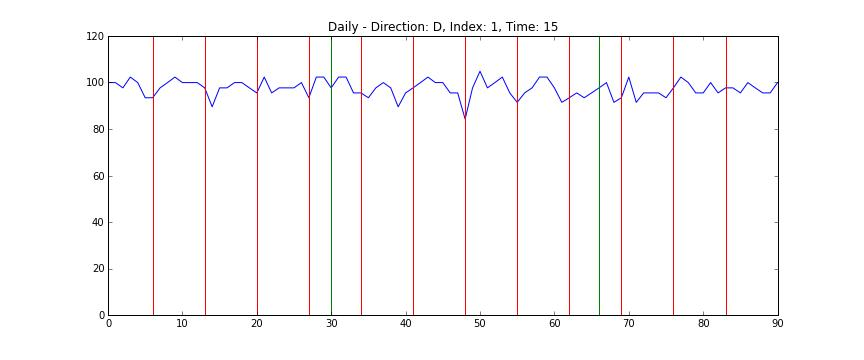
\includegraphics[width=0.85\paperwidth]{codesprint_015}
    \end{center}
}

\frame {
    \frametitle{데이터 분석}
    \framesubtitle{4월 1번 도로 하행선 19:20}
    \begin{center}
        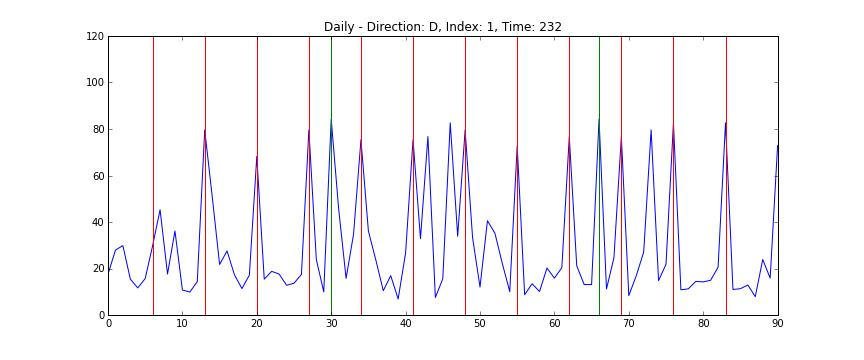
\includegraphics[width=0.85\paperwidth]{codesprint_232}
    \end{center}
}

\frame {
    \frametitle{가설}
    \begin{itemize}
        \item 주말과 주중 데이터는 서로 다른 규칙을 따른다
        \item 주중 데이터는 서로 같은 규칙을 따른다
    \end{itemize}
}

\frame {
    \frametitle{모델 생성}
    \begin{itemize}
        \item 데이터가 있으니
        \item 기계 학습 기법에 다 넣고
        \item 돌린다
        \item PROFIT???
    \end{itemize}
}

\frame {
    \frametitle{인과 관계}
    \begin{quote}
    통계 모델에 데이터를 집어 넣고 숫자를 뽑아내서 그 결과가 현실 세계의 올바른 표상이라고 무작정 받아들일 수 있으면 참 좋을 것이다.
    하지만 대부분의 경우, \textbf{인과 관계를 잘 고려하지 않으면 그럴 가망이 없는 결과만 얻을 뿐이다.}
    \begin{flushright}
    - Nate Silver
    \end{flushright}
    \end{quote}
}

\frame {
    \frametitle{생각하기}
    \begin{itemize}
        \item 지금 도로 상황이 보름 전의 도로 상황의 영향을 받는다?
        \item 말도 안 된다
        \item 아무리 좋은 기계 학습 기법을 사용해도 보름 전의 도로 상황으로 현재의 도로 상황을 예측하는 것은 힘들 것이다
    \end{itemize}
}

\frame {
    \frametitle{통계적 접근}
    \framesubtitle{모델}
    \begin{itemize}
        \item 하루 치 데이터를 생성하는 규칙이 있다고 가정하자
            \begin{itemize}
                \item 이 규칙을 알면 데이터를 그대로 생성하면 된다
            \end{itemize}
    \end{itemize}
}

\frame {
    \frametitle{통계적 접근}
    \framesubtitle{모델}
    \begin{itemize}
        \item 하루 치 데이터가 통째로 생성된다고 가정하자
            \begin{itemize}
                \item 앞뒤 시간은 서로 영향을 주고 받으니까
            \end{itemize}
            \begin{itemize}
            \item 하지만 이것은 어려운 문제
                \begin{itemize}
                    \item 전체적인 움직임과 국소적인 움직임을 모두 고려해야 한다
                    \item 어렵다
                \end{itemize}
            \end{itemize}
    \end{itemize}
}

\frame {
    \frametitle{통계적 접근}
    \framesubtitle{모델}
    \begin{itemize}
        \item 각 데이터는 모두 시간에 대해 독립적으로 생성된다고 가정하자
            \begin{itemize}
                \item 거짓말
                \item 하지만 이제 쉬운 문제가 된다
                \item 이제 변수 하나씩만 예측을 72,576 번 하면 된다
            \end{itemize}
    \end{itemize}
}

\frame {
    \frametitle{통계적 접근}
    \framesubtitle{예제}
    \begin{itemize}
        \item 내가 갖고 있는 하루하루 데이터가 하나하나 정답이라고 가정하자
        \item 내가 어떤 값을 제출하면 위의 데이터에서 평균적으로 가장 좋은 결과를 얻을 수 있을까?
    \end{itemize}

    \begin{eqnarray*}
        \displaystyle \argmin_{\hat{X}} \sum_{i} |\hat{X} - X_{i}|
    \end{eqnarray*}
    \begin{itemize}
        \item 중앙값이 이에 대한 최적해라는 이론이 있다
        \item An optimality property of median
    \end{itemize}
}

\frame {
    \frametitle{통계적 접근}
    \framesubtitle{결론}
    \begin{itemize}
        \item 주어진 채점 기준에 (\textbf{MAE}) 가장 적절한 값은 모든 데이터의 중앙값 (median)
        \item 앞서 언급한 \textbf{가정을 모두 적용}하면 이 데이터만 사용해서 얻을 수 있는 이론적 최적값
            \begin{itemize}
                \item 멋져 보이는 기계 학습 기법보다 더 좋은 결과가 보장됨
            \end{itemize}
    \end{itemize}
}

\frame {
    \frametitle{Result}
    \begin{center}
        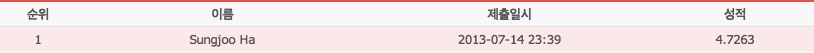
\includegraphics[width=0.85\paperwidth]{result}
    \end{center}
}


\frame {
    \frametitle{Future Work}
    \framesubtitle{요일별 중앙값 분포의 차이}
    \begin{center}
        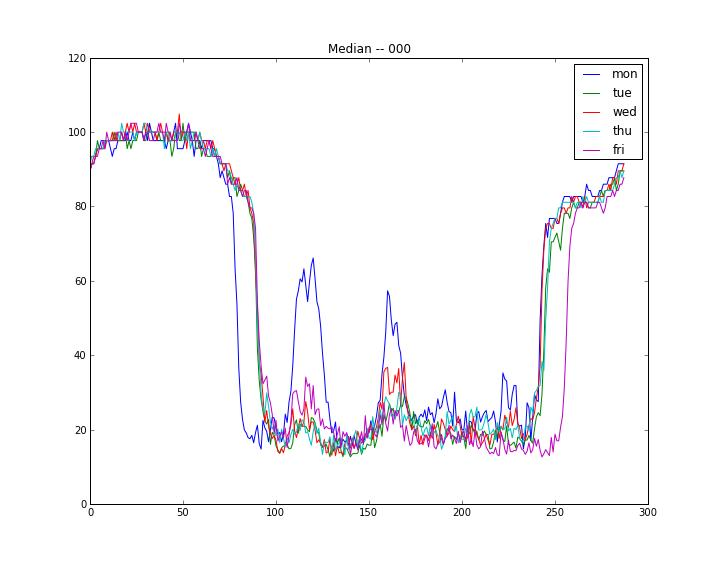
\includegraphics[height=0.75\paperheight]{codesprint_pm_000}
    \end{center}
}

\frame {
    \frametitle{Future Work}
    \framesubtitle{더 정교한 모델}
    \begin{itemize}
        \item 추가 데이터 사용
            \begin{itemize}
                \item 날씨, \ldots
                \item 더 많은 과거 데이터
            \end{itemize}
        \item ``진짜'' 베이지안 접근
            \begin{itemize}
                \item 데이터 생성 모델링
                \item Prior belief 설정
                \item Markov Chain Monte Carlo
                \item Posterior 샘플로부터 손실 함수의 기대값 최적화
                \item 블로그 글 참조
            \end{itemize}
        \item 모델 앙상블
    \end{itemize}
}

\frame {
    \frametitle{Reference}
    {\tiny
    \begin{itemize}
        \item The Signal and the Noise
        \item \url{http://blog.shurain.net/2013/07/code-sprint-2013-round-2.html}
        \item \url{http://blog.shurain.net/2013/08/code-sprint-2013-round-2-post-mortem.html}
        \item \url{http://en.wikipedia.org/wiki/Median}
    \end{itemize}
    }
}

\frame {
    \frametitle{Thank You!}
    \begin{center}

    {\Huge
    \url{bit.ly/codesprint2013r2}
    }

    \end{center}
}


\end{document}
